\documentclass[a4paper,fleqn,oneside]{cas-sc}

\usepackage[authoryear,longnamesfirst]{natbib}
\usepackage{amsmath,amssymb}
\usepackage{booktabs}
\usepackage{graphicx}
\usepackage{lmodern}
\usepackage{xcolor}
\usepackage{url}
\usepackage{amsthm}
\usepackage{algorithm}
\usepackage{tabularx}
% CAS expects key-value float options and unique hyperlink destinations.
\hypersetup{hypertexnames=false}
% Correct the CAS zero-width keyword overlay by adding balancing stretch.
% This fixes the box construction without suppressing layout diagnostics.
\ExplSyntaxOn
\RenewDocumentEnvironment{Abstract}{o}
{
  \group_begin:
  \IfNoValueTF{#1}{}{\tex_gdef:D\abstractname{#1}}
  \parindent=0pt
  \box_if_empty:NTF\g_stm_key_box
    {\leftskip=.35\textwidth}
    {
      \dim_gset:Nn\l_tmpa_dim{\box_ht:N\g_stm_key_box}
      \dim_gadd:Nn\l_tmpa_dim{\box_dp:N\g_stm_key_box}
      \leftskip=.35\textwidth
      \hspace*{-.35\textwidth}
      \noindent\hbox_to_wd:nn{0pt}{\box\g_stm_key_box\hss}
      \skip_vertical:n{-\l_tmpa_dim}
    }
  \noindent\abstractname\par
  \skip_vertical:n{-4pt}
  \noindent\rule{.65\textwidth}{.2pt}\par\footnotesize
  \ignorespaces\everypar{\parindent=1.5em}
}{\par\group_end:}
\ExplSyntaxOff
\renewcommand{\printorcid}{0000-0002-4008-0186}

%\usepackage{algorithmic}
\usepackage{algpseudocode}
\AtBeginDocument{\DeclareFontShape{T1}{lmr}{b}{it}{<-> ec-lmbo10}{}}
\hypersetup{pageanchor=false}
\usepackage{amsthm}

\theoremstyle{definition}
\newtheorem{example}{Example}
%\newtheorem{definition}{Definition}

\theoremstyle{plain}
%\newtheorem{proposition}{Proposition}
\newtheorem{theorem}{Theorem}
\newtheorem{lemma}{Lemma}
% The CAS front-matter machinery emits empty hyperlink anchors internally.
% Filter only that class-generated diagnostic; all other Hyperref warnings remain visible.
\makeatletter
\let\SCOriginalHyWarning\Hy@Warning
\renewcommand{\Hy@Warning}[1]{%
  \IfStrEq{#1}{Ignoring empty anchor}{}{\SCOriginalHyWarning{#1}}}
\makeatother

\newtheorem{proposition}{Proposition}
\newtheorem{definition}{Definition}
\newdefinition{remark}{Remark}
\newcommand{\Int}{\operatorname{Int}}
\newcommand{\Sub}{\operatorname{Sub}}
\newcommand{\cl}{\operatorname{cl}}
\newcommand{\Hard}{\mathsf{Hard}}
\newcommand{\sha}[4]{\texttt{#1\hspace{0pt}#2\hspace{0pt}#3\hspace{0pt}#4}}

\hypersetup{
  pdftitle={Beyond the Grand Coalition: Simplicial Heyting Semantics and Higher-Order Coalition Capacity in the European Parliament},
  pdfauthor={Alireza Pourmoslemi},
  pdfsubject={European Parliament: simplicial Heyting semantics and higher-order resilience},
  pdfkeywords={SC-Logic, European Parliament, Heyting negation, higher-order networks, modularity}
}

\begin{document}
\let\WriteBookmarks\relax
\def\floatpagepagefraction{0.8}
\def\textpagefraction{0.05}

\shorttitle{Graded simplicial negation in legislative coalitions}
\shortauthors{A. Pourmoslemi}

\title[mode=title]{Beyond the Grand Coalition: Simplicial Heyting Semantics and Higher-Order Coalition Capacity in the European Parliament}

\author[1]{Alireza Pourmoslemi}
\cormark[1]
\ead{a\_pourmoslemy@pnu.ac.ir}
\credit{Conceptualization, Methodology, Formal analysis, Software, Validation, Data curation, Visualization, Writing--original draft, Writing--review and editing}

\affiliation[1]{organization={Department of Mathematics, Payame Noor University},
  city={Tehran},
  country={Iran}}

\cortext[1]{Corresponding author}

\begin{abstract}
Pairwise party separation and higher-order legislative capacity need not move together. We apply simplicial Heyting semantics (SC-Logic) to European Parliament roll calls, tracking weighted Newman--Girvan party modularity and clique-based depth over thresholded co-Yes graphs. In the revised EP9 case study (2019--June 2022), modularity rises as the maximum face dimension falls at the selected local step. This is an exploratory finding: it does not identify the cause of the decline, and the location of the drop depends on the threshold mesh. Supplementary EP6 results from the 2004--2009 term, which use a legacy normalization and dimension limit, show the same direction without a comparable null test.
\end{abstract}
\begin{highlights}
\item Clique depth is tracked alongside party modularity in EP roll calls.
\item At one EP9 local step, modularity rises as maximum face dimension falls.
\item Party-aware nulls support the modularity contrast, not the depth drop.
\item The drop location depends on the threshold mesh.
\end{highlights}
\begin{keywords}
SC-Logic \sep simplicial Heyting semantics \sep European Parliament \sep higher-order networks \sep modularity \sep coalition structure
\end{keywords}
\maketitle
\hypersetup{pageanchor=true}
\pagestyle{plain}
\section{Introduction}\label{sec:introduction}

A legislature can be divided into clear political groups and still lose the
ability to form large coalitions across those groups. The two properties are
easy to confuse, because both are often summarised by a single number of
polarisation or cohesion. This paper argues that they should be measured
separately. We use weighted modularity $Q(\tau)$ to describe how strongly
members cluster into party groups, and the depth $d_{\max}(\tau)$ of a
threshold-dependent simplicial complex to describe how large a set of members
can be while still sharing a common vote. The claim is descriptive. Pairwise
modularity does not, on its own, characterise the coalition structure of a
chamber, and $d_{\max}$ records a dimension of it that $Q$ does not. We do not
treat modularity as a definition of polarisation, and neither quantity is
offered here as a measure of it.

We examine two windows of the European Parliament: the 6th term (2004--2009,
EP6) and the 9th term up to June 2022 (EP9). The windows differ in length,
membership and political context, so the comparison is a systematically
specified description rather than a controlled experiment. Roll calls are not
equivalent to laws, and member rows are not contemporaneous seat counts. We
therefore read the results as patterns under stated definitions and null
models, not as effects of particular historical events.

The formal setting is simplicial Heyting semantics (SC-Logic). A legislative
configuration is represented by a family of simplices that is partially
ordered by inclusion, and an explicitly chosen valuation lattice carries
Heyting operations. Higher-order representations can keep joint structures
that scalar graph summaries do not list directly \citep{BensonGleichLeskovec2016,
BattistonEtAl2020}. The construction has a cost: a clique in the threshold
graph need not be supported by any single roll call. For this reason we keep
three objects apart throughout: the observed support of Yes votes, the flag
complex generated by the threshold graph, and the poset of simplices on which
the semantics is evaluated.

Section~\ref{sec:framework} gives the construction and Section~\ref{sec:empirical_setup}
describes the data. Section~\ref{sec:results} separates local contrasts from
global associations, and Section~\ref{sec:discussion} discusses what the
results can and cannot support. Appendix~\ref{app:reproducibility} documents
the computational steps.

%% ============================================================
\section{Related work}
\label{sec:related}
%% ============================================================

The paper draws on five bodies of work: spatial models of roll-call voting,
empirical studies of the European Parliament, network measures of
polarisation and cohesion, higher-order and topological methods, and the
algebraic and political-theoretic background. For each we note what the work
measures and what it leaves open, because the contribution here depends on
that difference.

\subsection{Spatial models of legislative voting}

Much of the roll-call literature places legislators in a low-dimensional
policy space and infers their positions from how they vote.
\citet{PooleRosenthal1985} developed this approach for the U.S.\ Congress in
the NOMINATE family, and subsequent studies found that a small number of
dimensions accounts for most of the systematic variation in votes
\citep{PooleRosenthal1991,PooleRosenthal1997}. \citet{ClintonJackmanRivers2004}
estimate ideal points within a Bayesian framework, which gives an explicit
measure of uncertainty for each position. \citet{Carey2009} shows how
institutional arrangements shape voting cohesion, and his argument is a
reminder that group-level cohesion figures depend on the setting in which
they are produced.

These models describe proximity between pairs: two legislators are close when
they tend to vote alike. That information answers the question of who agrees
with whom. It does not directly say whether a given set of legislators can
support a motion together. The present paper turns to that second question by
looking at the size and depth of co-Yes coalitions, which are defined over
sets of members rather than over pairs.

\subsection{The European Parliament as an empirical site}

Studies of the European Parliament report that voting tends to follow
pan-European party groups more closely than national delegations.
\citet{HixNouryRoland2007} trace this pattern across successive terms and
describe how group cohesion developed over time. \citet{HixHoyland2011} set
these findings within a wider account of EU politics, in which conflict between
political groups structures parliamentary competition.
\citet{FarrellScully2007} look at the pull between constituency
obligations and party discipline in the behaviour of MEPs. That tension bears
on how group-level patterns should be read.

Two consequences follow for the present study. Party-group labels are a
natural reference partition for modularity, and this is the partition used in
Section~\ref{sec:setup}. Group structure also changes from one term to the
next, so label-based measures should be reported with their stability and not
as fixed features of the chamber. Our modularity results are therefore
conditional on the fixed label partition. They say nothing about whether that
partition is the best one available for the EP.

\subsection{Network approaches to polarisation and cohesion}

Network studies of legislatures usually build a graph in which members are
linked by similarity of voting. \citet{AndrisEtAl2015} apply this to U.S.\
House roll calls and report a long-run decline in cross-party cooperation.
The weight used here, the co-Yes weight $\omega(i,j)$, is computed from the
same kind of co-voting record. The difference is that we use it to build a
simplicial complex, not only a graph. Cosponsorship data offer a related network view of legislatures. \citet{Fowler2006} builds networks from bill cosponsorship in the U.S.\ House and Senate and uses them to describe connectedness among legislators. Such networks, like co-voting graphs, remain defined over pairs, which is the limitation the higher-order construction here addresses.

Modularity is the usual summary of how well a partition separates a network
into dense groups. \citet{GirvanNewman2002} proposed the divisive approach to
community structure, and \citet{NewmanGirvan2004} defined the index $Q$ used
in Section~\ref{sec:results}. \citet{Fortunato2010} reviews its known
weaknesses, among them the resolution limit and its dependence on the null
model. Both weaknesses carry over to the fixed-label variant used here.
\citet{BlondelEtAl2008} give a fast greedy method for maximising $Q$. We do not
optimise the partition. The Louvain method is cited only as the standard
reference for community detection, and the reported $Q$ is computed on fixed
party labels. \citet{ZhangWangZhang2007} study fuzzy community detection, in
which a node may belong to more than one community. We do not implement that
approach. The local contrast in Section~\ref{subsec:local} uses weighted
Newman--Girvan modularity on fixed labels. Network models of opinion formation also connect polarised states to the structure of the underlying network. \citet{PerezMartinezEtAl2023} study polarised opinion states in static networks under limited information. Our analysis is descriptive and does not model opinion dynamics, so we cite this work only as a pointer to dynamical explanations that the present data cannot test.

\subsection{Higher-order networks and simplicial topology}

A pairwise graph records interactions between two units at a time. Simplicial
complexes and hypergraphs can record interactions among larger groups.
\citet{BattistonEtAl2020} survey these frameworks and argue that some
structure disappears when interactions are projected onto pairwise edges.
\citet{BianconiBianconi2021} present simplicial complexes as models and discuss
their face-poset structure. \citet{BensonGleichLeskovec2016} show that
clustering on higher-order motifs can pick out organisation that pairwise
clustering misses. This is the motivation for the triangle-based statistic
$CI_{2,H}$ in Section~\ref{subsec:triangles}. \citet{BoccalettiEtAl2023} review the structure and dynamics of networks with higher-order interactions. \citet{ZhangLucasBattiston2023} compare hypergraphs and simplicial complexes and show that the choice between them can change collective dynamics. This is relevant here because the choice of a clique (simplicial) complex over a hypergraph is a modelling decision, and our depth results are conditional on it.
Simplicial models have also been used for dynamics on social networks. \citet{IacopiniEtAl2019} show that group interactions modelled by simplices change how contagion spreads. We do not model dynamics; we use the same simplicial representation only to describe static coalition capacity.

Topological data analysis gives another way to study structure across scales.
\citet{PataniaEtAl2017} apply persistent homology to collaboration networks
and follow how structure changes along a filtration. The threshold filtration
used here is similar in spirit, but we track the depth of the face poset and
not homological invariants. \citet{GiustiBassett2016} review topological
summaries of networks and point out that even zero-dimensional summaries, such
as connected components, carry information that edge density does not. This
is why $d_{\max}(\tau)$ is reported next to modularity and does not replace it.

\subsection{Lattice theory and Heyting semantics}

The algebraic setting is the Heyting algebra $\Sub(K_\tau)$ of subcomplexes
ordered by inclusion. The general theory of Heyting algebras that arise from
frames and toposes is treated in \citet{Johnstone1982}.
\citet{MacLaneMoerdijk1992} connect the subobject classifier of a presheaf
topos with lattices of sieves, and this is the viewpoint from which the
semantics of Section~\ref{sec:framework} is read.

The stage-local negation $\neg_\tau\varphi=\Int(K_\tau\setminus\varphi)$ is the
Heyting pseudocomplement in this lattice. \citet{Lawvere1991} discusses the
dual co-Heyting structure in the setting of certain toposes. We do not use the
dual, and mention it only to mark the boundary of the construction. The graded reading of negation in Section~\ref{subsec:hns} comes from the SC-Logic framework \citep{Pourmoslemi2026Semantics}; a broader treatment of topological approaches to logic and uncertainty appears in \citet{Pourmoslemi2026Truth}. We cite both for the reading of negation alone, not for any empirical result.


\subsection{Political theory}

Section~\ref{sec:discussion} relies on several traditions. \citet{Habermas1996}
grounds democratic legitimacy in communicative reason, and treats
coalition-building across difference as central to deliberative politics.
\citet{Arendt1958HumanCondition} places political action in the space between
plural actors, which gives us a way to read the distance between pairwise
proximity and higher-order coalition capacity. \citet{Mouffe2000,Mouffe2013}
argue that agonistic pluralism describes democratic conflict more realistically
than the consensus ideal. We use these works only as interpretive context.
Section~\ref{subsec:political} considers what algebraic measures can and cannot
establish about normative questions. \citet{Schmitt2007} frames the political through the friend--enemy distinction, which Mouffe's agonistic account engages critically. We mention it only because it is the contrast against which agonistic pluralism is defined.

\subsection{Positioning}

Put together, the literatures leave a particular gap. Spatial models describe
pairwise proximity. The EP studies document group-level structure but do not
measure coalition capacity above the level of pairs. The network and
topological work offers multi-scale tools, and to our knowledge these have not
been applied to roll-call coalitions in the form used here. The paper defines
a coalition capacity on sets of members, follows its depth along a threshold
filtration, and compares that depth with modularity computed on fixed party
labels. The conclusions are limited to what these computations show under the
stated null models and sensitivity checks.

\section{Mathematical framework: simplicial Heyting semantics}\label{sec:framework}
\subsection{Observed coalitions and threshold capacity}
Let $A_{ir}\in\{-1,0,+1\}$ encode No, abstention/non-participation, and Yes for member row $i$ and roll call $r$. Abstention and absence remain distinct raw codes but are excluded from both Yes and strict No witnesses. For $U_r=\{i:A_{ir}=+1\}$, define
\begin{equation}
K^{\mathrm{obs}}=\{\varnothing\ne\sigma\subseteq V:\exists r,\ \sigma\subseteq U_r\}.
\end{equation}
This downward closure encodes shared assent, not deliberative quality. Define
\begin{equation}
\omega_{\mathrm{EP9}}(i,j)=\begin{cases}\dfrac{\sum_r\mathbf1\{A_{ir}=A_{jr}=+1\}}{c_{ij}},&c_{ij}\geq20,\\0,&c_{ij}<20,\end{cases}\quad
G_\tau=(V,\{\{i,j\}:\omega(i,j)\geq\tau\}).
\end{equation}
Here $c_{ij}=\sum_r P_{ir}P_{jr}$, where $P_{ir}=1$ only for a recorded Yes, No, or Abstain decision; absence is not presence. This separate indicator is required because the ternary zero alone does not distinguish abstention from absence. EP9 uses this co-presence denominator, with observed sensitivity analyses at minimum counts 10 and 50. EP6 retains the legacy denominator of all roll calls; cross-term density comparisons therefore use different normalizations. All vertices, including isolates, are retained. Flag capacity $F_\tau=\mathrm{Cl}(G_\tau)$ differs from $K^{\mathrm{obs}}_\tau=K^{\mathrm{obs}}\cap F_\tau$: pairwise assent can arise on different roll calls. Increasing $\tau$ gives a decreasing filtration, not a temporal history.
\subsection{Depth and computational bounds}
For a nonempty finite complex, the longest chain of nonempty faces has length $d_{\max}+1$. The depth computation records
\begin{equation}
D(\tau)=d_{\max}(\tau)+1,\qquad \mathrm{BD}_n(\tau)=d_{\max}(\tau).
\end{equation}
Here $\mathrm{BD}_n$ is a notational alias for $d_{\max}$, not a logical completeness or inferential-length theorem. The legacy EP6 rows retain the dimension-15 limit; EP6 v3 (co-presence) runs uncapped, with 17 of 41 thresholds unfinished, reported as bounds. EP9 uses uncapped maximum-clique search: certified rows report exact dimension, while unfinished searches report lower and upper bounds, not a substituted exact value. The EP9 search budget is 10 seconds on $0.38$--$0.52$ and within $0.02$ of the selected drop, and 0.5 seconds elsewhere. Isolated vertices have dimension zero and depth one.
\subsection{Distinct Heyting algebras}\label{subsec:heyting}
The finite distributive lattice $\Sub(K)$ of downward-closed subcomplexes is a Heyting algebra \citep{Johnstone1982,Pourmoslemi2026Semantics}:
\begin{equation}
L\Rightarrow M=\bigcup\{C\in\Sub(K):C\cap L\subseteq M\},\quad \neg L=L\Rightarrow\varnothing.
\end{equation}
It must not be identified with the algebra of upsets on $P_K=(K,\subseteq)$. For that Alexandrov topology, open sets are coface-closed:
\begin{equation}
\neg_H U=\{\sigma:\uparrow\!\sigma\cap U=\varnothing\},\quad
\neg_H\neg_H U=\operatorname{int}(P_K\setminus\neg_H U).
\end{equation}
A boundary defined by set difference need not be a subcomplex or upset.
\begin{proposition}[Antitonicity]
Within either specified Heyting algebra, $U\subseteq W$ implies $\neg W\subseteq\neg U$.
\end{proposition}
\begin{proof}
Every admissible element disjoint from $W$ is disjoint from $U$. Taking the greatest such element gives the inclusion; strictness is not guaranteed.
\end{proof}
Negation is graded by changing ambient complexes and valuations, not by assigning numerical intensities to individual opposition.
\subsection{Stage-local HNS and group traces}\label{sec:hns}
On the 1-dimensional face poset of $G_\tau$, let $U_v=\uparrow\!v$ contain $v$ and its incident edges. Then
\begin{equation}
\text{HNS}(\tau)=\frac{|\{v:\deg(v)>0,\ \neg_H\neg_H U_v\ne U_v\}|}{|\{v:\deg(v)>0\}|}.
\end{equation}

The implementation records zero when no vertex is active. The statistic has an algebraic meaning. In a Heyting algebra, $\neg\neg a=a$ holds for every element exactly when the algebra is Boolean, and $\neg\neg a\ne a$ witnesses that $a$ lies outside the Boolean core $\{a:\neg\neg a=a\}$. Each defective $U_v$ is therefore a certified witness of non-Booleanity, and $\text{HNS}(\tau)$ is the fraction of tested principal upsets that are witnesses. Here double negation adds precisely the degree-one neighbors of $v$, so a defective active vertex is adjacent to a leaf; this identity is specific to the 1-dimensional poset. Consequently $\text{HNS}(\tau)>0$ proves that the algebra is not Boolean, whereas $\text{HNS}(\tau)=0$ does not, because only the sets $U_v$ are tested. Accordingly, $1-\text{HNS}$ is a descriptive ratio over these valuations and not a measure of the full algebra. Treating HNS as a graded quantity, we use it only to compare stages, not to assign a numerical intensity to any actor.

For group vertices $G$, set $N_\tau(G)=\{v\notin G:\exists g\in G,\{v,g\}\in E_\tau\}$. The implemented vertex traces are
\begin{align}
Z_G&=(V\setminus G)\setminus N_\tau(G),\\
Z_G^{(2)}&=(V\setminus Z_G)\setminus N_\tau(Z_G),\quad
\operatorname{defect}_G=|Z_G^{(2)}\setminus G|.
\end{align}
These are traces of group-upset negation and double negation, not induced-complement negation in $\Sub(K)$.
\subsection{Triangle channels and modularity}\label{sec:ci}\label{subsec:triangles}
A flag triangle has a strict No witness iff all three members vote No on at least one common roll call. The separate-channel statistic is
\begin{equation}
CI_{2,\mathrm{cross}}=1-\frac{\#\{\text{flag triangles with a shared No witness}\}}{f_2(F_\tau)}.
\end{equation}
It is set to one for zero triangles, with counts retained to flag that convention. Separate channels do not imply statistical independence. The separately specified $CI_{2,H}(G)$ is the density of graph triangles meeting both $G$ and $N_\tau(G)$ among all possible triples in their union meeting both sets; it is undefined for zero denominator.

Weighted party modularity is
\begin{equation}
Q(\tau)=\frac1{2W}\sum_{i,j}\left(w_{ij}-\frac{k_i k_j}{2W}\right)\mathbf1\{g_i=g_j\},
\end{equation}
where $w_{ij}=\omega(i,j)\mathbf1\{\omega(i,j)\geq\tau\}$, $k_i=\sum_jw_{ij}$ and $2W=\sum_i k_i$. Edgeless graphs have conventional $Q=0$. This is the Newman--Girvan functional \citep{NewmanGirvan2004}, evaluated on fixed party labels, not optimized communities or a verified distinct Zhang modularity. Comparison with fuzzy community detection \citep{ZhangWangZhang2007} is representational, not an algorithmic replication.
\section{Empirical setup and computational pipeline}\label{sec:empirical_setup}\label{sec:setup}
\subsection{Corpus and provenance}
Individual votes are taken from the VoteWatch Europe roll-call-vote workbooks for EP6 (extract of 13 June 2022) and EP9 (extract of 22 June 2022); accompanying workbooks provide act metadata only. The EP9 records end in June 2022. We refer to that window as EP9 (2019--2022), although the institutional term continued through 2024.

Table~\ref{tab:ep_summary} reports membership-row counts rather than simultaneous chamber sizes. Historical labels are harmonized to EPP, Socialists (PES/S\&D), Liberals (ALDE/Renew), Greens/EFA, the Left, conservative/sovereigntist families, and non-attached members. UEN-to-conservative harmonization is an analytical mapping, not organizational identity. Static grouping can obscure changes of affiliation and membership turnover.
\begin{table}[pos=t]\centering\small
\caption{Audited local EP corpora. EP9 ends in June 2022. Density is the edge density of $G_{0.50}$. Rows marked ``co-presence'' use the co-presence denominator with at least 20 joint observations; these rows are comparable across terms. Rows marked ``legacy'' use the original all-roll-call denominator and dimension-15 search limit, and are retained historical results that are not comparable to EP9. Capped rows (EP6 only) do not identify the true maximum dimension. Co-presence EP6 values are taken from the archived \texttt{results\_v3} EP6 outputs. For EP6, the legacy and co-presence density values differ because they use different denominators; only the co-presence values are comparable with EP9.}

\label{tab:ep_summary}
\begin{tabular}{lrr}\toprule
Attribute & EP6 & EP9\\\midrule
Recorded membership rows & 940 & 811\\
Roll calls in aligned matrix & 6,199 & 13,459\\
Harmonized political groups (excluding UNKNOWN) & 8 & 8\\
Recorded Yes decisions & 2,207,437 & 5,349,743\\
Mean affirmative coalition size & 356.095661 & 397.484434\\
Maximum reported dimension (capped; legacy EP6) & 15 & ---\\
Edge density at $\tau=0.50$ (legacy; not comparable) & 0.004173748 & ---\\
Edge density at $\tau=0.50$ (co-presence) & 0.285664 & 0.275170\\
Modularity $Q$ at $\tau=0.50$ (co-presence) & 0.278700 & 0.169221\\
Last threshold at dimension ceiling (EP6 only) & 0.52 & ---\\
First edgeless threshold (EP6 legacy) & 0.66 & 0.86\\\bottomrule
\end{tabular}
\end{table}
\subsection{Execution and audit}
The mesh comprises 41 thresholds $\tau\in\{0.10,0.12,\ldots,0.90\}$. Exact Yes pair counts generate the graphs. Trajectory, poset-depth, and local-contrast records are aligned by threshold. Mean affirmative coalition sizes are counts of Yes votes per roll call.



A row is artifact-flagged when its edge count is at most five, active-vertex count at most ten, or component count equals edge count. The recorded component count includes isolates. Summary statistics are evaluated with and without flagged rows. Fixed-topology group-label permutations form a negative control: HNS does not depend on these labels.
\section{Empirical Results}\label{sec:results}\label{sec:experiments}
\subsection{EP6 and EP9 trajectory dynamics}
Figure~\ref{fig:ep-depth} separates the historical dimension-limited EP6 trajectory from revised, uncapped EP9 results. On the 0.02 mesh EP9 has 35 certified exact rows and six timeouts, at $\tau=0.14,0.20,0.22,0.24,0.26,0.28$. Exact dimension is 697 at $0.10$, 387 at $0.44$, and 302 at $0.50$; the first edgeless threshold is $0.86$. Bounds, not point estimates, describe unfinished searches. Different weight denominators and search guarantees preclude a direct capped EP6--uncapped EP9 persistence comparison.
\begin{figure}[pos=htbp]\centering
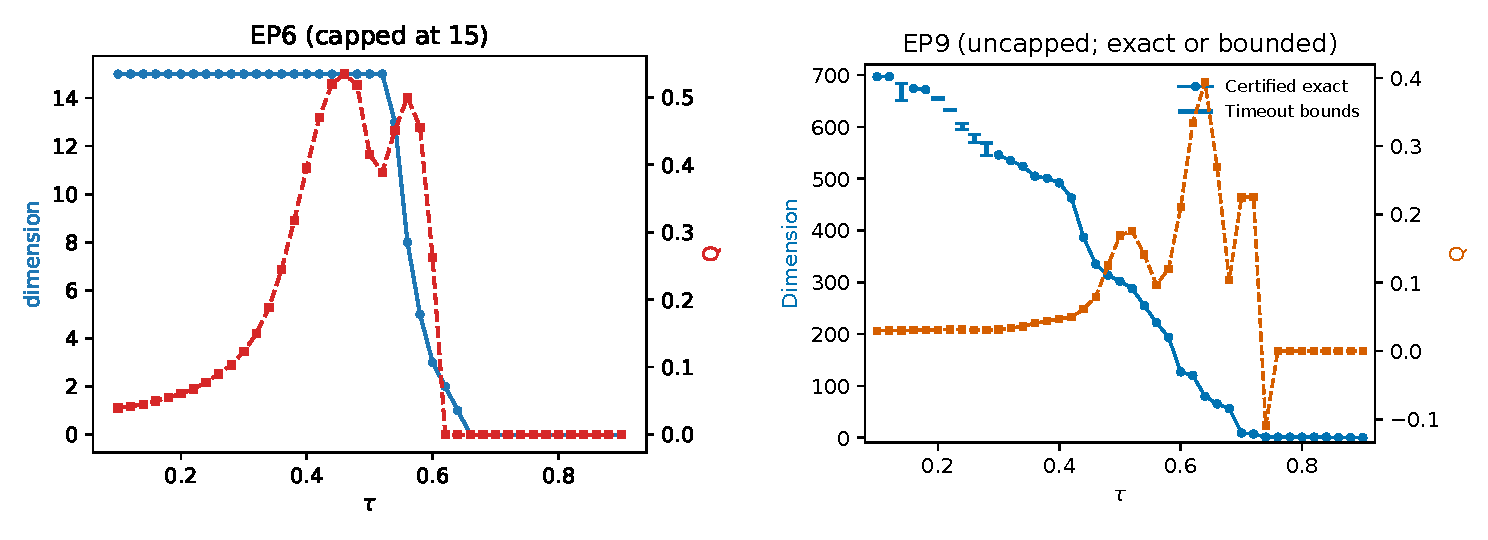
\includegraphics[width=0.9\textwidth]{sc_logic_figures/ep_depth_Q_v8.pdf}
\caption{Historical EP6 capped dimension (left) and revised EP9 uncapped dimension with weighted Newman--Girvan modularity (right). EP9 markers denote certified values; vertical intervals give lower/upper bounds for six timeouts at $\tau=0.14,0.20,0.22,0.24,0.26,0.28$. Poset depth equals dimension plus one; $\mathrm{BD}_n$ equals dimension. EP6 and EP9 use different weight denominators.}
\label{fig:ep-depth}\end{figure}
\subsection{Local modularity contrasts and global associations}\label{subsec:local}
On the EP9 0.02 mesh, the certified largest drop is $0.42\to0.44$: exact dimension falls from 463 to 387 ($\Delta d=-76$), while $Q$ increases from 0.049523124 to 0.061155409 ($\Delta Q=0.011632285$). On the 0.01 mesh, the largest certified drop is $0.42\to0.43$ ($\Delta d=-47$, $\Delta Q=0.004700461$), but its global optimality is unverified because other searches timed out. On the 0.05 mesh, the certified largest drop is $0.40\to0.45$ ($\Delta d=-135$, $\Delta Q=0.022355365$). These are mesh-dependent local steps, not a mesh-invariant transition. Figure~\ref{fig:ep-local} displays the revised local contrasts.

For 2000 contiguous block-bootstrap resamples (seed 42), depth is an uncapped fixed-order two-start greedy lower-bound envelope, not exact dimension. At block length 50, the 95\% intervals are $[-0.614798,0.226416]$ for Pearson correlation and $[-0.534703,0.112423]$ for Spearman correlation. These refer to approximate depth and include zero; no directional global association is established. At $0.42\to0.44$, the $\Delta Q$ interval is $[0.002819469,0.020088002]$ and the approximate-depth increment interval is $[-72,-6]$. The approximate-depth point increment is $-38$, unlike the exact observed $-76$. Threshold dependence and search approximation limit interpretation.
\begin{figure}[pos=htbp]\centering
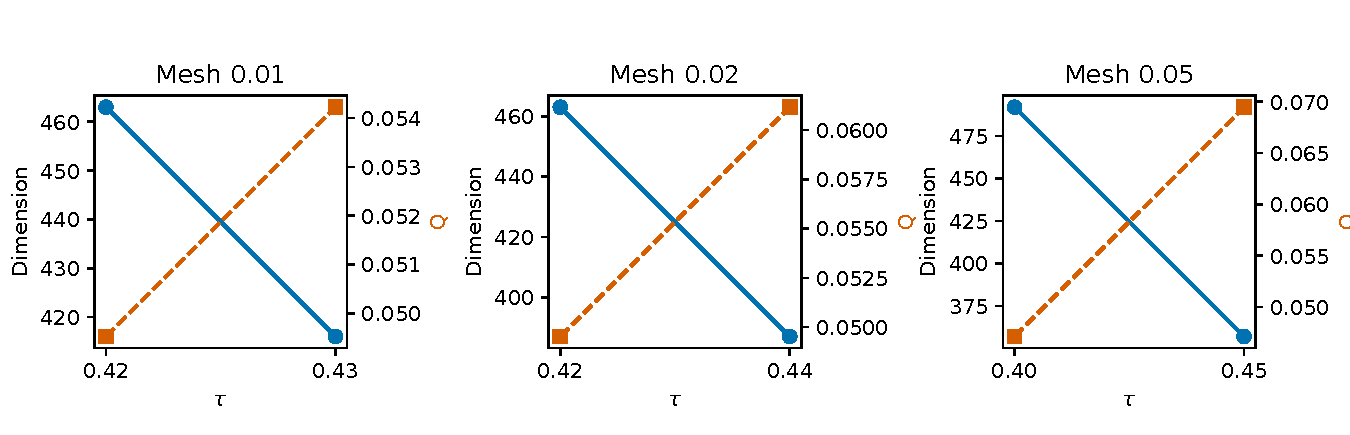
\includegraphics[width=0.9\textwidth]{sc_logic_figures/ep_local_v8.pdf}
\caption{Revised EP9 mesh-specific selected steps. Each pair shows certified endpoint dimensions and weighted Newman--Girvan modularity. On the 0.01 mesh the largest certified drop need not be the global maximum over unfinished searches.}
\label{fig:ep-local}\end{figure}

\subsection{HNS: stage-local defects and sparse-tail artifacts}\label{subsec:hns}
HNS evaluates double negation independently at each threshold. It has no memory across thresholds, estimates no change point, and does not detect phase transitions. Peaks may co-occur with sparse configurations without identifying a cause. Figure~\ref{fig:ep-hns} marks rows requiring this qualification.

The EP6 maximum at $\tau=0.64$ is exactly one disconnected dyad plus 938 isolated vertices. Both active vertices are defective, giving HNS equal to one. This sparse-tail artifact is not compelling evidence of maximal political multipolarity. With artifacts included, EP6 mean, median, and peak HNS are 0.054656, 0.005690, and 1.000000; after exclusion, 0.040035, 0.018975, and 0.285714. EP9 values are 0.007802, 0.001901, and 0.078947 with artifacts, and 0.010319, 0.003110, and 0.078947 without. The EP9 peak occurs at $\tau=0.66$ and is not flagged.

At those peaks, 1,000 group-label permutations with seed 42 leave HNS invariant. The null standard deviation is zero and the empirical upper-tail probability is one. A standardized $z$ score is undefined for this degenerate null; the stored zero is a reporting convention, not evidence of significance. A group-dependent statistic would be required for an informative label-permutation test.
\begin{figure}[pos=htbp]\centering
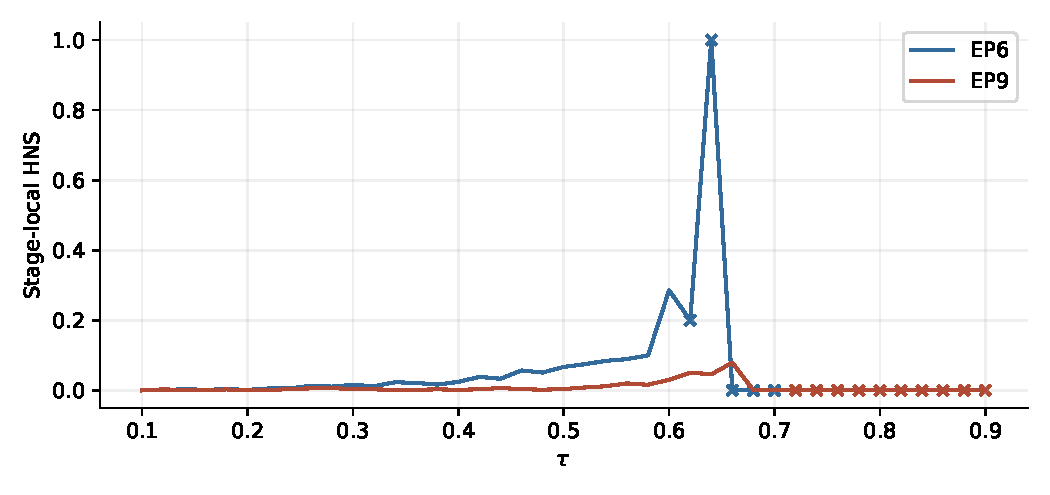
\includegraphics[width=0.9\textwidth]{sc_logic_figures/ep_hns_artifact_audit.pdf}
\caption{Stage-local HNS. Crosses denote artifact-flagged rows. The EP6 peak at 0.64 is generated by one dyad, not an identified political transition.}
\label{fig:ep-hns}\end{figure}

\subsection{Party-aware null for EP9}\label{subsec:party-null}
The EP9 party-aware null uses fixed input, seed 42, and 1000 draws, permuting Yes/No/Abstain states within party and roll call while preserving member presence. Two UNKNOWN members remain their own group. For any exact statistic $T$, the one-sided upper-tail Monte Carlo probability is
\begin{equation}
p_T=\frac{1+\sum_{b=1}^{1000}\mathbf1\{T_b\geq T_{\mathrm{obs}}\}}{1001}.
\end{equation}
The implementation compares $Q_b\geq Q_{\mathrm{obs}}-10^{-12}$. For bounded depth, let observed bounds be $[l_o,u_o]$ and draw bounds $[l_b,u_b]$. The reported lower probability counts $l_b\geq u_o$ and the upper probability counts $u_b\geq l_o$, each with the same plus-one correction. Ambiguous comparisons are possible but not guaranteed exceedances. No multiple-testing correction is applied.

At tested thresholds $0.40$--$0.46$, observed modularity exceeds all null draws; this is not true at $0.50$. Depth upper-tail intervals do not establish exceptional depth loss: these stagewise tests do not directly test $\Delta d$. Table~\ref{tab:vote-null} gives all revised EP9 probabilities.
\subsection{Historical fixed-margin reference}\label{subsec:vote-null}
The earlier EP6 fixed-margin vote-matrix experiment used 200 MCMC draws (seed 42) preserving each member's nonzero vote count and each roll call's Yes/No counts. Its dimension statistic was limited to 15, and convergence was not established. EP6 null draws were not rerun in results\_v3. Figure~\ref{fig:vote-null} retains that historical reference only; its obsolete EP9 panel is removed. No capped fixed-margin EP9 result is compared with the revised uncapped observations.
\begin{table}[pos=htbp]\centering\small
\caption{Revised EP9 party-aware null (1000 draws, seed 42). Depth probabilities are bounded upper-tail probabilities; ambiguous counts reflect unresolved depth comparisons, not missing draws. Multiple testing is uncorrected.}\label{tab:vote-null}
\begin{tabular}{rrrrr}\toprule
$\tau$ & $Q_{\mathrm{obs}}$ & $p_Q$ & $[p_d^{\mathrm{lower}},p_d^{\mathrm{upper}}]$ & Ambiguous\\\midrule
0.40 & 0.047121590 & 0.000999001 & $[0.811188811,1.000000000]$ & 189 \\
0.42 & 0.049523124 & 0.000999001 & $[0.933066933,1.000000000]$ & 67 \\
0.44 & 0.061155409 & 0.000999001 & $[1.000000000,1.000000000]$ & 0 \\
0.46 & 0.079100574 & 0.000999001 & $[1.000000000,1.000000000]$ & 0 \\
0.50 & 0.169220537 & 1.000000000 & $[0.996003996,1.000000000]$ & 4 \\
\bottomrule\end{tabular}\end{table}
\begin{figure}[pos=htbp]\centering
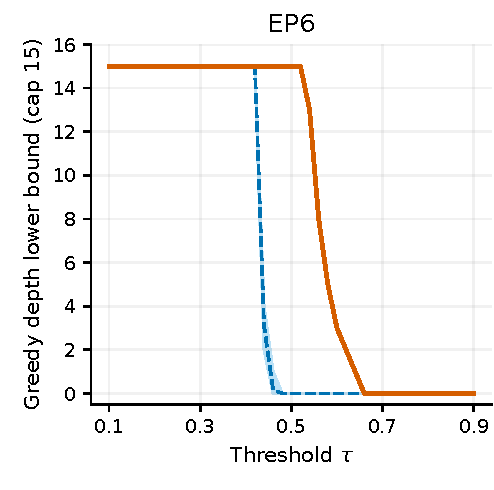
\includegraphics[width=0.85\textwidth]{sc_logic_figures/fig5_null_model_dmax_ep6_legacy.pdf}
\caption{Historical EP6 fixed-margin reference only: observed dimension-limited greedy depth and pointwise null band from 200 MCMC draws. EP6 was not rerun in results\_v3. The obsolete EP9 panel is excluded; revised EP9 inference is in Table~\ref{tab:vote-null}.}\label{fig:vote-null}
\end{figure}

\section{Discussion}\label{sec:discussion}
\subsection{Separation is not higher-order resilience}
Rising $Q(\tau)$ may accompany a loss of higher-order cross-party structure. One possible account is that, as weaker cross-party ties are removed, surviving edges concentrate within parties, raising modularity while reducing the size of cliques and face chains. The present analysis does not test this account and does not identify a causal effect of political behavior. Group-pure fragments need not preserve the full network's cross-party higher-order configurations; conversely, a large clique does not establish shared deliberative justification.

Joint reporting is therefore warranted. The results do not make modularity mathematically defective: $Q$ answers a different question and its limitations require care \citep{Fortunato2010}. Neither dimension nor its decline establishes non-collapsibility under simplicial collapses, homological persistence, or a hard ideological core. Those claims require additional invariants.
\subsection{Interpretive note: the political space-between}\label{subsec:political}
The following is a theoretical interpretation, not a finding. If thresholding removes cross-party bridging configurations, increased party separation can coexist with less room for structurally shared positions. Deliberative accounts hold that legitimacy cannot be reduced to density or a scalar consensus score \citep{Habermas1996}, and Arendtian accounts locate political action in the plurality of actors appearing to one another \citep{Arendt1958HumanCondition}. Agonistic pluralism, by contrast, holds that common coalitions need not erase legitimate disagreement \citep{Mouffe2000,Mouffe2013}. The combinatorial result is only that clique-based chains shorten as $d_{\max}$ falls; it does not prove reduced inferential competence, rights, or legitimacy, and it is not a measure of the willingness to dissent.
\section{Scope, specification, and methodological limitations}\label{sec:limitations}
The revised EP9 co-presence denominator excludes absence but includes recorded abstention, with minimum 20 joint observations. EP6 legacy rows use the original denominator and dimension-15 cap; the co-presence rows use the revised denominator.

Six of 41 EP9 observed searches time out, at $\tau=0.14,0.20,0.22,0.24,0.26,0.28$; their exact depths are unknown within reported bounds. Null searches also time out, requiring probability intervals and ambiguous counts. The selected drop is mesh-dependent: $0.42\to0.43$, $0.42\to0.44$, and $0.40\to0.45$ for meshes 0.01, 0.02, and 0.05, respectively; global optimality on the finest mesh remains unverified. Bootstrap results use approximate greedy depth, not exact maximum cliques, for all 2000 resamples at block lengths 20, 50, and 100.

Party-aware tests are stagewise, one-sided, and uncorrected for multiple testing; they do not directly test a depth-increment null or establish causation. Two UNKNOWN members remain a separate group rather than being assigned a party. The revised EP9 party-aware null supplements the historical EP6 fixed-margin null; EP6 was not rerun in results\_v3. HNS and triangle-channel sections retain earlier diagnostics and were not recomputed on corrected EP9 input in this revision. The modularity implemented here is Newman--Girvan only, not a distinct Zhang algorithm.

EP9 coverage ends in June 2022; only two legislative windows are studied. Static grouping can hide party switching. No causal claim about Brexit or the pandemic is supported. Yes and No channels share roll calls and are not independent. Flag capacity is not observed joint-vote support; dimension alone does not establish homological persistence, political competence, or democratic legitimacy.

Downset and upset semantics yield different negations. Neither HNS equal to zero nor its Boolean-core ratio proves that the full face-poset algebra is Boolean. Stage-local HNS and invariant label permutations cannot detect phase transitions or establish political significance.

\section{Conclusion}\label{sec:conclusion}
In revised EP9 observations, Newman--Girvan party modularity rises while higher-order clique capacity falls at the selected local step. Modularity exceeds the party-aware null at the tested thresholds from $0.40$ to $0.46$, but not at $0.50$. Bounded depth tests do not establish a depth drop beyond the null, and they do not directly test increments. Drop location depends on threshold mesh; unfinished searches and approximate bootstrap depth remain explicit limitations. The legacy EP6 results are not an equivalent uncapped comparison. SC-Logic supplies proposition-relative semantics, not a causal or normative inference about democratic quality.
\section*{Declaration of competing interest}
The author declares that they have no known competing financial interests or personal relationships that could have appeared to influence the work reported in this paper.

\section*{Funding}
This research did not receive any specific grant from funding agencies in the public, commercial, or not-for-profit sectors.

\section*{Data and code availability}

The raw VoteWatch Europe roll-call-vote workbooks used in this study (EP6 extract of 13~June~2022; EP9 extract of 22~June~2022) are not redistributed here, as they remain the property of VoteWatch Europe.

The derived summaries, analysis code, and party-aware null-model outputs are
publicly available at \url{https://github.com/pourmoslemy/EP-SC-Logic} and are
archived on Zenodo (DOI: \href{https://doi.org/10.5281/zenodo.23643385}{10.5281/zenodo.23643385}).
The archive does not include the raw VoteWatch workbooks, the corrected input arrays,
or individual member-level vote records. All code is released under the MIT License.
Access to the raw workbooks is subject to the data provider's terms. The archive
documents the pipeline and the derived results reported here.


\appendix
\section{Reproducibility record}\label{app:reproducibility}
The numerical sources for the revised EP9 results are the \texttt{results\_v3} output files archived in the repository (release v0.1.3, directory \texttt{results/}); EP6 co-presence summaries are in \texttt{results/EP6/}. Fixed-input Yes totals were computed from the corrected input, which is not redistributed; the resulting totals are reported in the derived summaries archived in the repository.
 All 41 default thresholds retain search status and lower and upper depth bounds. Mesh-specific increments, null ambiguity, and approximate bootstrap intervals are reported as separate records. Seed 42 is used for the stored null and bootstrap experiments. Historical EP6 and protected HNS diagnostics are retained without a claim of rerunning them on revised input.

\paragraph{Conventions.}
All-threshold correlations include edgeless rows and use average ranks for Spearman ties. $CI_{2,\mathrm{cross}}=1$ is used for the no-triangle case; $CI_{2,H}$ is missing when no admissible triples exist. HNS is set to zero when there are no active vertices. A stored degenerate-null value of $z=0$ denotes undefined standardization and is not a valid Gaussian score. Static grouping and member identifiers require further audit before any individual-level interpretation.

\par\medskip
\printcredits
\bibliographystyle{cas-model2-names}
\bibliography{references_v5}
\end{document}
